\documentclass[a4paper,12pt]{article}

\usepackage[T1,T2A]{fontenc}        % Кодировки шрифтов
\usepackage[utf8]{inputenc}         % Кодировка текста
\usepackage[english,russian]{babel} % Подключение поддержки языков

\usepackage{amsthm}                 % Оформление теорем
\usepackage{amstext}                % Текстовые вставки в формулы
\usepackage{amsfonts}               % Математические шрифты

\newtheorem*{ther}{Теорема}
\newtheorem*{defi}{Определение}
\usepackage[pdftex]{graphicx}       % Вставка картинок
\graphicspath{{pictures/}}            % Стандартный путь к картинкам
\newcommand{\eps}{\varepsilon}
\newtheorem*{Consequence}{Следствие}

\begin{document}

    \section*{Задача 11}

    Покажите, что последовательность $(1 + \frac{1}{n})^n$ имеет предел.

    \begin{ther}[О трёх последовательностях]
        Если последовательности 
        $\{ x_{n}\}$, $ \{ y_{n} \} $, $ \{ z_{n} \}$
        таковы, что  $x_{n} \leq y_{n} \leq z_{n}$ для всех 
        $n \geq N_{0}$,  $\lim\limits_{n\to \infty }x_{n}=\lim\limits_{n\to \infty }z_{n}=a$, то последовательность  $ \{ y_{n} \}$ сходится и  $\lim\limits_{n\to \infty }y_{n}=a$.
    \end{ther}

    \begin{proof}
        По определению предела для любого $\eps > 0$ найдутся номера $N_{1}=N_{1}(\eps)$ и  $N_{2}=N_{2}(\eps)$ такие, что  $x_{n}\in U_{\eps }(a)$ при всех  $n\geq N_{1}$ и  $z_{n}\in U_{\eps }(a)$ при всех  $n\geq N_{2}$. Отсюда и из условия $x_{n}\leq y_{n}\leq z_{n}$ для всех  $n \geq N_{0}$  следует,
        \begin{center}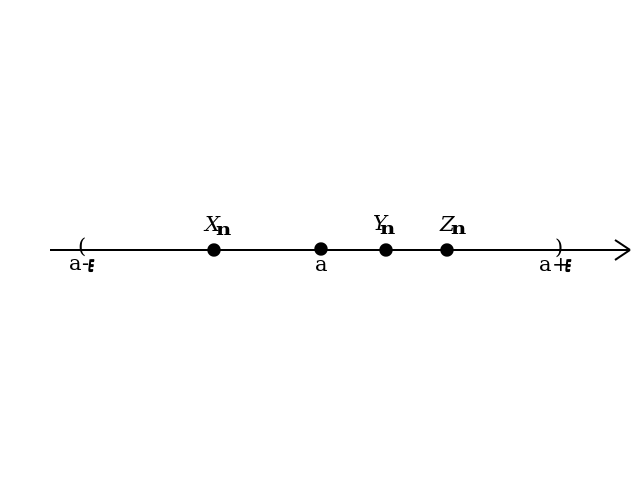
\includegraphics[scale=0.4]{1.png}\end{center}
        что при всех  $n\geq N$,  где $N = max \left ( N_{0},N_{1},N_{2} \right )$, выполняется условие  $y_{n}\in U_{\varepsilon }(a)$. Это означает, что существует  $\lim\limits_{n\rightarrow \infty }y_{n}=a$.
    \end{proof}

    \begin{ther}
        Если  $\lim\limits_{n\rightarrow \infty }x_{n}=a,~ \lim\limits_{n\rightarrow \infty }x_{n}=b$, причем  $a<b$, то
        $$\exists N_{0} :\forall n\geq N_{0} \rightarrow x_{n}< y_{n}.$$
    \end{ther}

    \begin{proof}
        Выберем  $\varepsilon > 0$  таким, чтобы $\varepsilon$-окрестности  точек а и b не пересекались (возьмем, например,  $\varepsilon =\frac{\left ( b-a \right )}{3}>0)$.  Согласно определению предела по заданному $\varepsilon$ можно найти номера  $N_{1}$ и $N_{2}$ такие, что $x_{n}\in U_{\varepsilon}(a)$ при всех   $n\geq N_{1}$ и    $y_{n}\in U_{\varepsilon}(b)$ при всех   $n\geq N_{2}$. Пусть  $N_{0}= max\left ( N, N_{2} \right )$. Тогда при всех  $n\geq N_{0}$ выполняются неравенства

        $$x_{n}<a+\varepsilon <b-\varepsilon < y_{n}$$

        откуда следует утверждение

        $$\exists N_{0} :\forall n\geq N_{0} \rightarrow x_{n}< y_{n}.$$

    \end{proof}

    \begin{Consequence}
        Если  $\lim\limits_{n\rightarrow \infty }x_{n}=a$, $\lim\limits_{n\rightarrow \infty }y_{n}=b$, и  $\forall n\in \mathbb{N}\rightarrow x_{n}\geq y_{n}$  то

        $$a\geq b.$$
    \end{Consequence}

    \begin{proof}
        Предположим, что неравенство   $a\geq b$ не выполняется. Тогда $a < b$
        и по предыдущей теореме справедливо утверждение

        $$\exists N_{0} :\forall n\geq N_{0} \rightarrow x_{n}< y_{n},$$

        которое противоречит  условию

        $$\forall n\in \mathbb{N}\rightarrow x_{n}\geq y_{n}.$$

        Поэтому должно выполняться неравенство  $a\geq b$.
    \end{proof}
\end{document}